\newpage
\section*{Appendix C: User Guide}

In this Appendix we will illustrate main functionalities for two types of users:
\begin{itemize}
    \item Human Resources Employee
    \item Applicant
\end{itemize}

\subsection*{Human Resources}

The HR user should write a title and a description for the job, specify if the introductory video is required or not. And at last he should add list of questions to the job specifying for each of them if it is required or not. The HR user should at least add one question or an error will result and job creation will not be performed. Fig \ref{fig:create_job_correct} shows an example of error-free job creation.


\begin{figure}[h!]
\centering
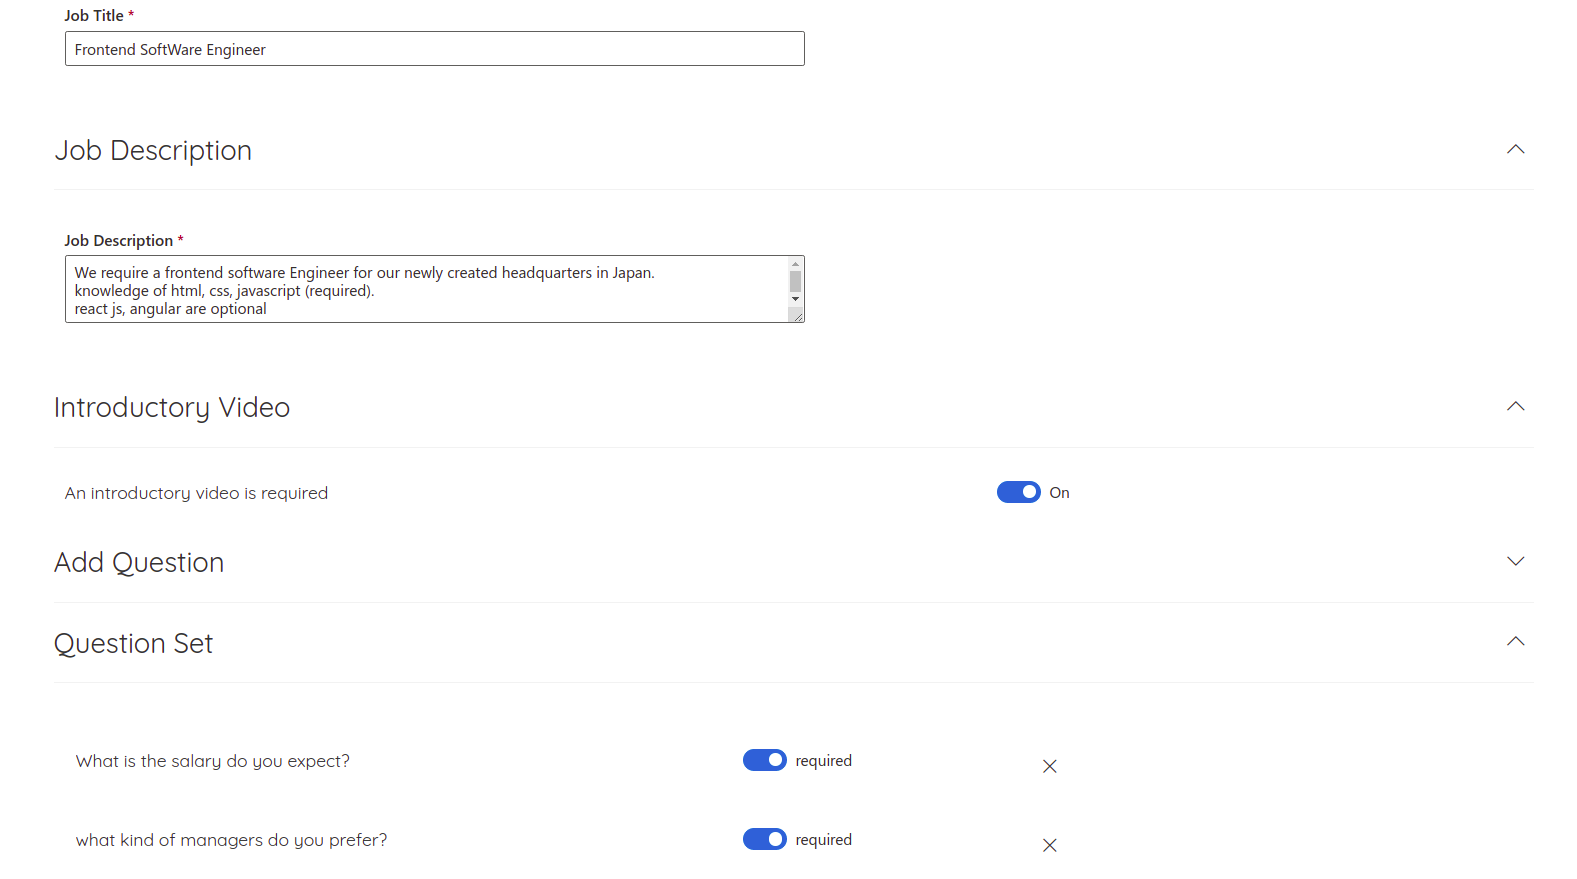
\includegraphics[width=10cm,height=6cm, frame]{images/create.png}
\caption{An error-free example of new job creation}
\label{fig:create_job_correct}
\end{figure}


The HR can manipulate applications of users, filter them and sort them according to the CV Ranker, the date of application or names. Also he can gain insights about their behavior and personality. Moreover he can view applicants' applications or profiles. As shown in fig  \ref{fig:view_insights}.


\begin{figure}[h!]
\centering
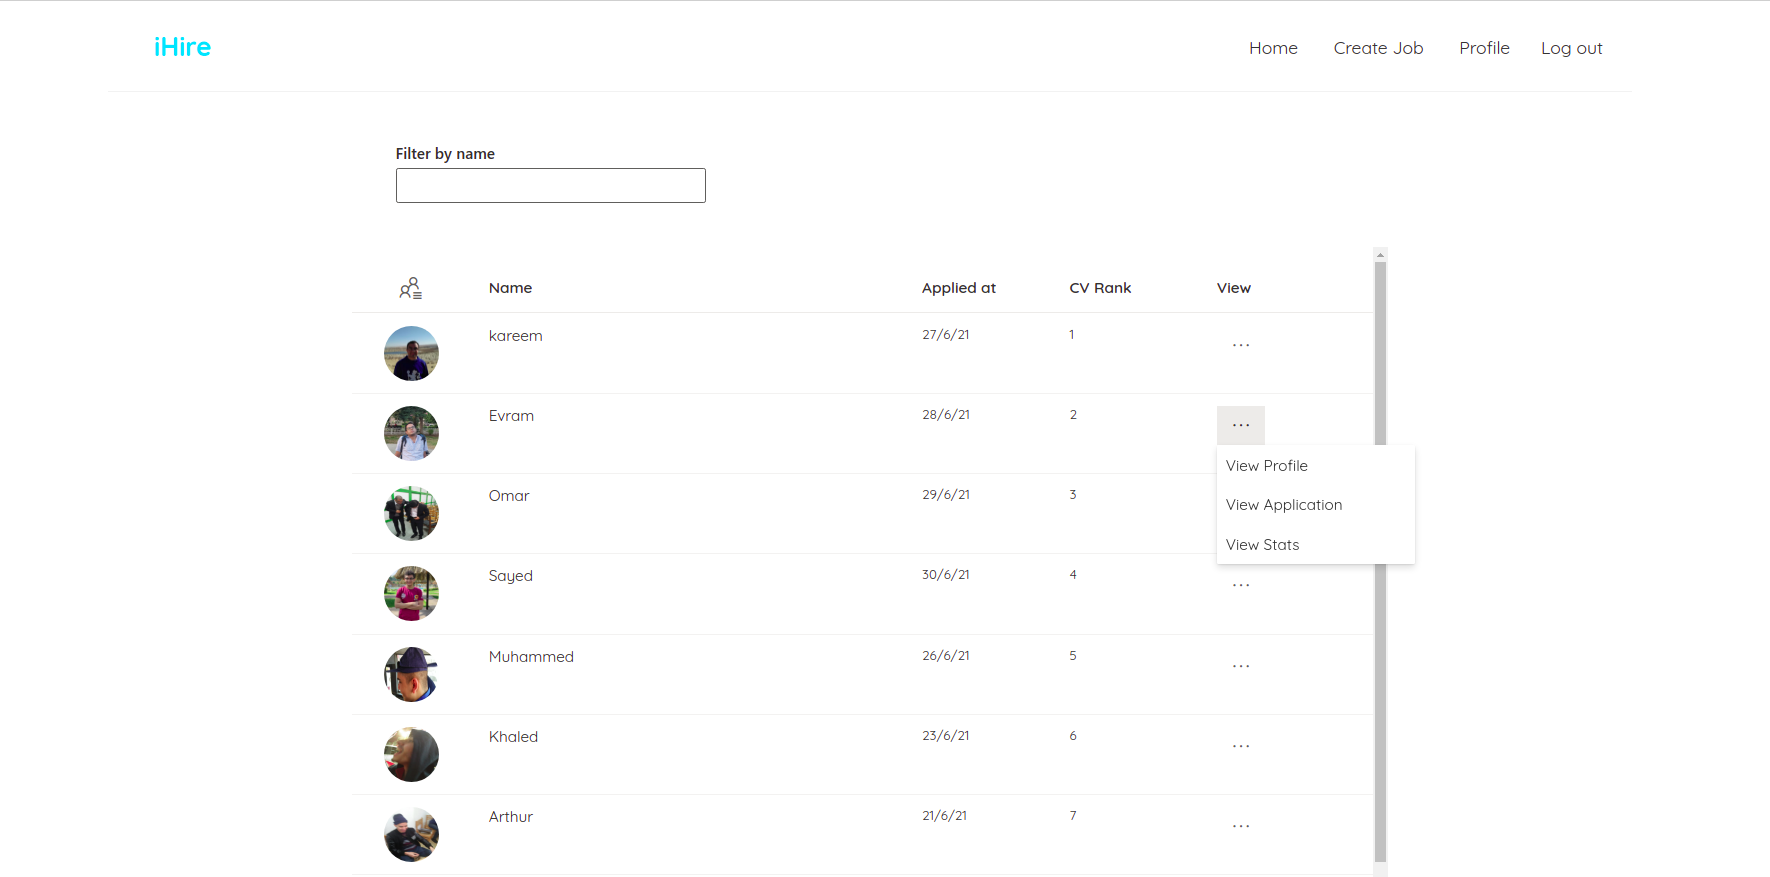
\includegraphics[width=10cm,height=6cm, frame]{images/User Interface/view.png}
\caption{view and manipulate applications}
\label{fig:view_insights}
\end{figure}



\subsection*{Applicant}

An applicant to fulfill the application, he should upload his resume, an introductory video if required, and he should answer the required questions. If he dropped one of this implications the application will not be fulfilled. A user can edit his application several times if he wants. Fig \ref{fig:apply_job_correct} shows an error-free application example.


\begin{figure}[h!]
\centering
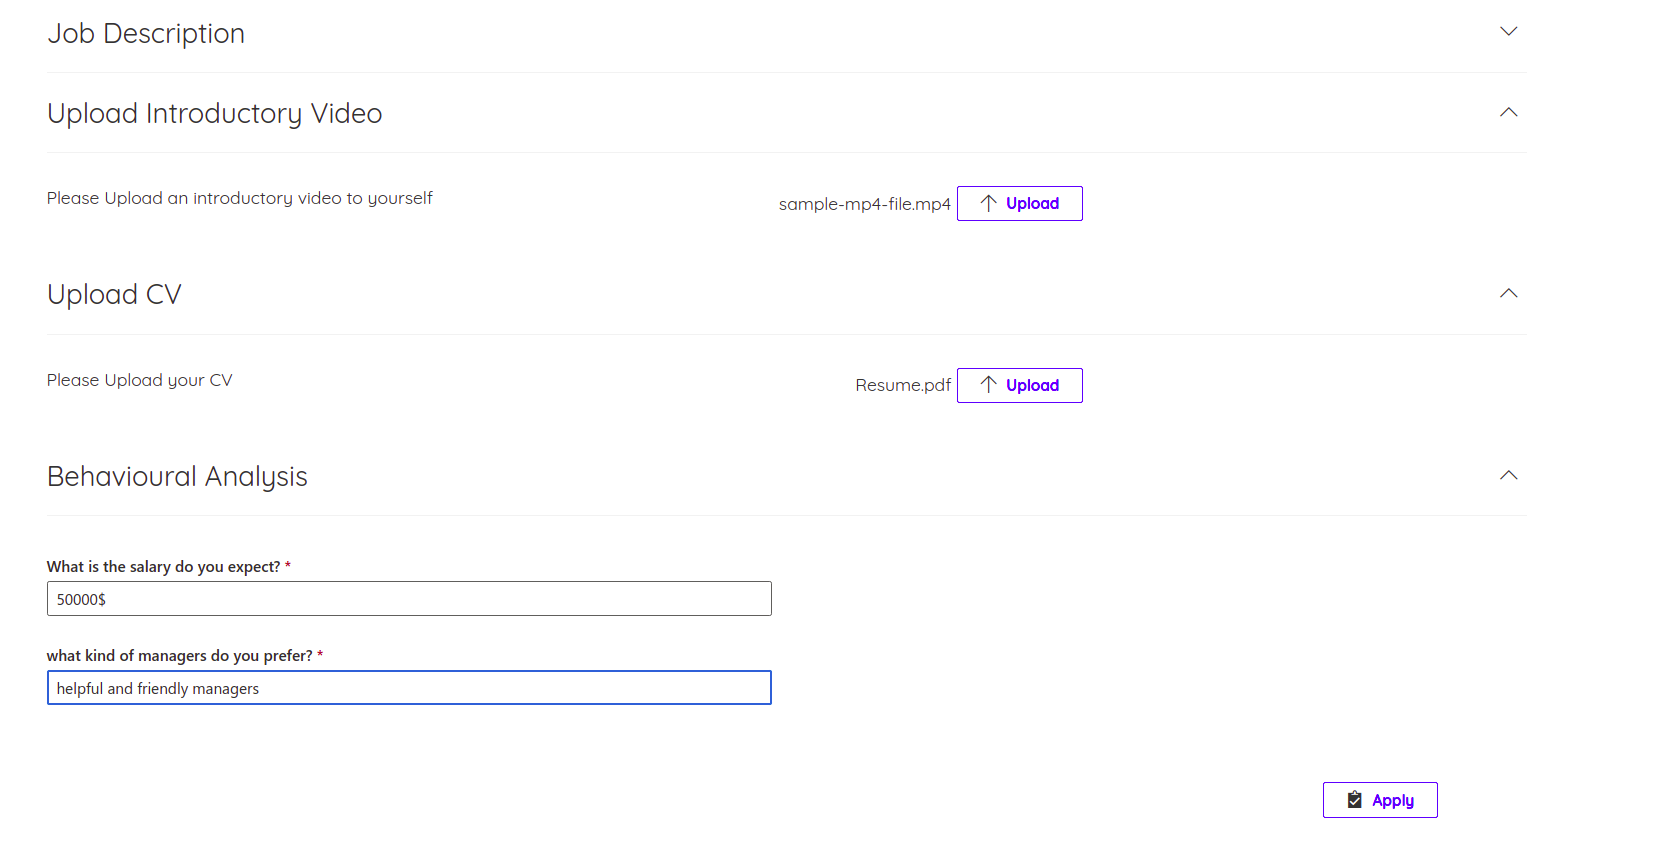
\includegraphics[width=10cm,height=6cm, frame]{images/apply.png}
\caption{An error-free example of user application on a job}
\label{fig:apply_job_correct}
\end{figure}

